\documentclass[letterpaper,11pt,twoside]{article}
\usepackage{amsmath,amssymb,amsfonts,amsthm}
\usepackage[margin=1.0in]{geometry}
\usepackage{fancyhdr, lastpage}
\usepackage[pdftex]{graphicx}
\usepackage{hyperref}
\hypersetup{
    colorlinks,
    citecolor={black},
    linkcolor={black},
    urlcolor={black},
    bookmarksnumbered,
    pdfstartview={FitH},
    pdfpagemode={UseOutlines},
    pdftitle={Creepy - Project Report},
    pdfauthor={Travis Hall, Brittany Thompson and Bhadresh Patel},
    pdfsubject={CS 453 Project}
}

\setlength{\parskip}{0.5ex}
\pagestyle{fancy}
\setlength{\headheight}{14.0pt}
\fancyhead{}
\fancyfoot{}
\fancyhead[RO,RE] {Project Report: \emph{Creepy - Data Cleanser}}
\fancyfoot[LO,LE] {CS 453: Project 2 - Data Preparation}
\fancyfoot[RO,RE] {Page \thepage\ of \pageref{LastPage}}
\renewcommand{\headrulewidth}{0.5pt}
\renewcommand{\footrulewidth}{0.5pt}

\begin{document}

%%%%%%%%%% Title Page %%%%%%%%%%%%%%%%%%%%%%%%%%%%%%%%%%%%%%%%%%%%%%%%%%%%%%%%%%
\begin{titlepage}
   \begin{center}
       {\Large \textbf{CS 453: Project 2 - Data Preparation}}\\[0.5cm]
       {\Large \textbf{Project Report}}\\[3.0cm]

       {\rule{\linewidth}{0.5mm}} \\[0.5cm]
       {\Huge \textbf{Creepy - Data Cleanser}}\\[0.4cm] 
       {\rule{\linewidth}{0.5mm}} \\[2.0cm]

       \textbf{Travis Hall}\\
       \texttt{trvs.hll@gmail.com}\\[0.5cm]
       \textbf{Brittany Thompson}\\
       \texttt{miller317@gmail.com}\\[0.5cm]
       \textbf{Bhadresh Patel}\\
       \texttt{bhadresh@wsu.edu}\\[0.5cm]

       \vfill
       Washington State University Vancouver\\
       October 03, 2010
   \end{center}
\end{titlepage}

\begin{abstract}
The main goal of this project is to design and implement data preparation or data cleansing stage of the search engine. We already collected small collection of pages via the web crawler in our first project. We will be removing all unnecessary portions in the document collection through a combined process of (i) tag-stripping, (ii) tokenizing, (iii) stopping, and (iv) stemming. Additionally, we will be preparing a document graph for link analysis. 
\end{abstract}

\section{Overview}
In this project, \emph{Creepy} is designed to prepare the document collection that was crawled by the crawler for the further stages of the search engine \emph{i.e.} cleanse documents. The documents crawled by the crawler are typically not in a plain text. Instead, most of them are in HTML format and can also be in other well know formats like Word, Powerpoint, PDF etc. These documents needs to be convert into text plus some metadata for the further stage of the search engine. In project 1, we tweaked our crawler to crawl documents that are in plain text or HTML format only. Conversion of other formats to plain text is rather complicated and is beyond the scope of this project.    

\begin{figure}[htb]
 \centering
 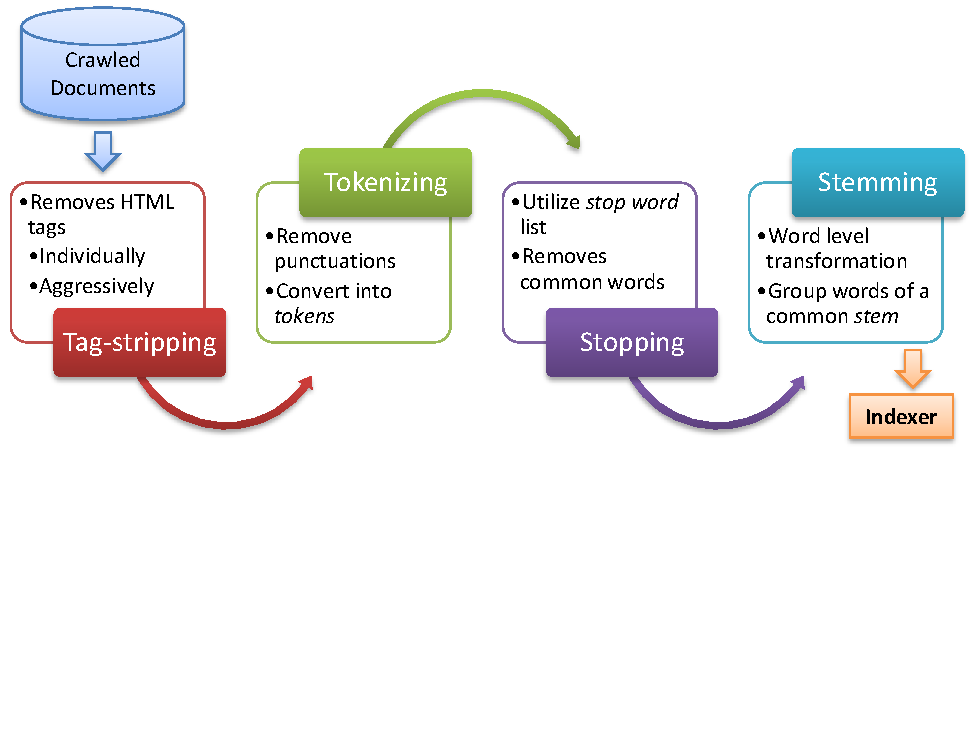
\includegraphics[trim=0.0in 2.00in 0.0in 0.0in, clip, page=1]{figures.pdf}
 \caption{Data Cleansing}
 \label{fig:data_cleansing}
\end{figure}

The task of data cleansing process is to take the collection of documents already crawled by the crawler and convert them into sequence of text \emph{tokens} for the indexer component of the search engine. The cleansing process will generate the cleansed document through a combined process of (i) tag-stripping, (ii) tokenizing, (iii) stopping, and (iv) stemming as illustrated in the figure~\ref{fig:data_cleansing}.

\section{XML Document Graph}
The first step in creating our XML document graph was to construct a document type definition (DTD) to base it off. The first few elements of the DTD were practically a given: (i) we need an element that will carry all of the documents as children, this we called \texttt{docstore}; and (ii) we need an element for storing the document information, fittingly, we named this one \texttt{doc}.

The design decisions after that were predominantly guided by the amount of information we needed. In order to create a graph structure, each document needed to have fields for tracking which documents linked to it and which documents are linked from it. However, we did not really need the full document descriptions of those links. Instead, all we needed were the document's URLs and their IDs (the filename on the local system). As such, we chose to create these elements as a list, where their children were very simple entities with a pair of attributes (URL and ID) and nothing more. As such, \texttt{to} and \texttt{from} contain a list of \texttt{page}s.

Creating the graph itself was not terribly complex. For this component, named \emph{Rucksack}, I chose to use Ruby, being most comfortable with it and needing to complete it quickly. The majority of the work is done in the \texttt{DocStore} class, where it imports a map-file (\texttt{pid\_map.dat}) and creates the structure of \texttt{Doc} and \texttt{Page} classes. In the interest of saving memory with larger map files, each structure is created only once and stored within a hash based on its URL. As the map is rigged together or as entities are fully defined, it simply updates the fields.

Finally, each class is given a \texttt{\#to\_xml} method that utilizes Ruby's \emph{Builder} Gem (library). This means that each component can be converted directly into an XML description individually. The overall construction of the DTD-compliant structure is handled by \texttt{DocStore\#to\_xml}.

In the interest of verifying that components worked, there were two small testing scripts written for \texttt{Doc} and \texttt{DocStore}. While not terribly in-depth, they helped to smooth out several bugs with the map-rigging and the XML construction.

\section{XML Validator}
In order to make sure \emph{Rucksack} created a valid tree based on our DTD, we wanted to write a XML-validator for doing so. Unfortunately, this process is extremely complex. While efforts were made to create a validator (which can be seen under \texttt{lib/validator/parser.rb}) the task was simply too large to complete in the remaining time. For comparison, \emph{libxml2}, a standard and popular C library for handling XML, and also the library that most validators wind up utilizing (for example \emph{libxml-ruby} and \emph{libxml2} for Python, PHP, and Perl), took 15,000 lines just for validating the XML syntax alone (which included parsing DTD/Doctype declarations but not constructing the tree). The actual DTD validation added another 7,000 lines on top of that.

Our implementation in Ruby will validate a small portion of the XML syntax, however due to time constraints it was not possible to complete the full validator. Instead, so that we could still make sure \emph{Rucksack} was constructing XML that was valid by our DTD, we leveraged \emph{libxml} and a set of bindings for Ruby to complete the validation. This can be seen in \emph{validate.rb} at the top level of the project.

In retrospect, starting the parser from the bottom-up would have made for a less daunting approach. Establishing the terminals and then moving upwards into the non-terminals would have allowed more flexibility in the code. Unfortunately, as my first parser, I did not have enough experience to recognize this.

For reference, the XML 1.0 language description used can be found here: \url{http://www.w3.org/TR/REC-xml/}

\section{Tag-stripping}
The first task in the data cleansing process is to recognize the structural elements of the document and remove them. This process is referred to as \emph{tag-stripping}. Document structure is often specified by a markup language, for example HTML is used for specifying the structure of web pages. The tag-stripping component uses knowledge of the syntax of the HTML language to identify the structure of the document. In HTML, \emph{tags} are used to define document elements. These tags does not add any value for the search engine and they are removed at this stage. There is two types of tag stripping (i) aggressively; and (ii) \emph{individually}; that can be applied to the document collection. Tag-stripping is performed on the document collection that is crawled by the crawler.

\subsection{Aggressive tag-stripping} 
Aggressive tag-stripping removes the whole HTML element \emph{i.e.} removes tags and its content. There are certain tags in HTML page that is used only for structural purpose or for dynamic scripting only. These HTML elements can be removed fully since it does not contribute any relevant information for the search. For example, \verb|<script type="text/javascript">functionCall();</script>| would be fully removed by the tag-stripping component. We selected following HTML tags that are aggressively removed from the document: script, style, object, embed, applet, noframes, and noscript. 

\subsection{Individual tag-stripping}
Individual tag-stripping only removes the tags and its attributes from the HTML element and leaves any content intact that occurs between the opening and closing tag. For example, \\\verb|<h1 style="font-size:14px;">My page title</h1>| will become \verb|My page title| after removing individual tags. After the aggressive tag-stripping is applied to the document, individual tag-stripping is applied to remove any tags appear in the document. After this stage, the resulting document will only contain plain text that does not have any structural elements of the document. 

\subsection{Implementation}
\begin{table}[htb]
\centering
\begin{tabular}{|p{\textwidth}|}
\hline
\begin{verbatim}
<html xmlns="http://www.w3.org/1999/xhtml" lang="en">
  <head>
    <title>WSU Vancouver - Engineering and Computer Science</title>
    <link rel="shortcuticon" href="/sites/all/themes/departments/favicon.ico" 
         type="image/x−icon" />
    <script type="text/JavaScript" language="JavaScript">
        var id=3; functionCall(id);
    </script>
    <style type="text/css">
        .field-content {margin:4px;}
    </style>
  </head>
<body>
  <div class="field−content">
    <p>The School of Engineering and Computer Science (ENCS) is an academic unit
    of the WSU College of Engineering and Architecture that houses the
    engineering and computer science programs located at
    <a href="http://www.vancouver.wsu.edu">WSU Vancouver</a>.
    The School offers ABET accredited Bachelor of Science degrees in computer
    science and mechanical engineering.</p>
  </div>
</body>
</html>
\end{verbatim}\\
\hline
\end{tabular}
\caption{Sample HTML document}
\label{tab:samplepage}
\end{table}

\begin{table}[htb]
\centering
\begin{tabular}{|p{\textwidth}|}
\hline
\begin{verbatim}
 
   
     WSU Vancouver - Engineering and Computer Science 
     
     
     
   
 
   
     The School of Engineering and Computer Science (ENCS) is an academic unit
    of the WSU College of Engineering and Architecture that houses the
    engineering and computer science programs located at
     WSU Vancouver .
    The School offers ABET accredited Bachelor of Science degrees in computer
    science and mechanical engineering. 
   
 
 


\end{verbatim}\\
\hline
\end{tabular}
\caption{Sample HTML document after tag-stripping}
\label{tab:samplepage_stripped}
\end{table}

The implementation of tag-stripping is done in Python. There are some Python modules available that allows stripping tags from the HTML document, for example, HTMLParser, htmllib, Beautiful Soup and sgmllib. In our initial experiments, we notice that most of these modules removes tags quite effectively when the HTML page is well-formed---syntactically valid HTML document. But they failed to remove some tags if the document is not well-formed. Since, web pages are inherently error prone document that does not necessarily follow the standards. So we were not able to use existing modules of Python for our tag-stripping component. We wrote our own module that uses regular expression to remove any tags. The regular expressions are written such that it does not care about well-formed HTML elements and still remove all the tags. The table~\ref{tab:samplepage} shows sample HTML document and after removing tags using the tag-stripping component the generated document is shown in table~\ref{tab:samplepage_stripped}.

\section{Tokenizing}
\emph{Tokenizing} is the process of forming term or token from the sequence of characters in a document. Thus, tokenizing converts most of the document content to search-able tokens. Tokenizer takes the document that was generated by the tag-stripping component as input and generates a new document that contains only tokens. At this stage, we assume that the tag-stripping component removed any text that was structural part of the document and leaves text that is actual content of the document. The design of our tokenizer consist of three step process as described below.
\begin{description}
	\item [Case folding] This is the simplest step in which all uppercase letters are converted to lowercase. 
	\item [Remove punctuations] In this step we remove all the punctuation characters from the document. We considered \verb !"#$%&\'()*+,-./:;<=>?@[\\]^_`{|}~  as the punctuation characters that are removed from the document.
	\item [Generate tokens] The last step is to generate tokens, in this step multiple spaces, new line, tab etc.. are removed. The resulting document will contain all the terms separated by single space.
\end{description}

\begin{table}[htb]
\centering
\begin{tabular}{|p{\textwidth}|}
\hline
\begin{verbatim}
wsu vancouver engineering and computer science the school of engineering and
computer science encs is an academic unit of the wsu college of engineering
and architecture that houses the engineering and computer science programs
located at wsu vancouver the school offers abet accredited bachelor of
science degrees in computer science and mechanical engineering
\end{verbatim}\\
\hline
\end{tabular}
\caption{Tokens generated by tokenizer for the sample HTML document}
\label{tab:samplepage_tokenized}
\end{table}

At the end of the three step process of tokenizer we save the generated tokens into new document that is used for further steps in data cleansing process. For example, the table~\ref{tab:samplepage_tokenized} shows the tokens generated (each token is separated by sapce) by the tokenizer for the sample document produced by tag-stripping component as shown in the table~\ref{tab:samplepage_stripped}. We note that, the design of the tokenizer is kept simple and flexible, the same rules would be applied to the search query in the query transformation component. Hence, all the punctuations and tokens would be treated in same manner to the query and it should result in appropriate match to the index terms. 

\section{Stopping}

\section{Stemming}


\section{Roles}
\begin{description}
 \item[Travis Hall] Link analysis graph and XML validator.
 \item[Brittany Miller] Stopping and stemming.
 \item[Bhadresh Patel] Tag-stripping and tokenizing.
\end{description}

\section{Test Environment}
For testing/production purpose, we set up a machine instance on Amazon EC2. The instance id of the machine is \texttt{i-7d1e0d17}. The source code is checked out at \texttt{/home/ubuntu/creepy/}.

\section{Usage Guide}
The process for generating cleanse document is sequential as illustrated in the figure~\ref{fig:data_cleansing}, so here are the steps for using the program in same sequence.

\begin{enumerate}
	\item Crawl the web	
	\begin{verbatim}
	$ python creepy.py -S storage -c seed.txt -T 2500 -N 300
	\end{verbatim}
	
	\item XML Document Graph
	Rucksack requires two RubyGems be installed (both of which come standard with later versions of Ruby):
	\begin{verbatim}
	  $ gem install hpricot
	  $ gem install builder
	\end{verbatim}
	For default options:
	\begin{verbatim}
	  $ ruby rucksack.rb pid_map.dat
	\end{verbatim}
	For the current production environment:
	\begin{verbatim}
	  $ ruby rucksack.rb -a crawled storage/pid_map.dat -o map.xml
	\end{verbatim}
	
	\item Validation
	The validator requires one RubyGem be installed, as well as libxml and zlib.
	On OS X with MacPorts installed, libxml and zlib can be installed with:
	\begin{verbatim}
	  $ port install libxml2
	\end{verbatim}
	On Debian linux:
	\begin{verbatim}
	  $ apt-get install libxml2 libxml2-dev
	\end{verbatim}
	Installing libxml-ruby:
	\begin{verbatim}
	  $ gem install libxml-ruby
	\end{verbatim}
	Running:
	\begin{verbatim}
	  $ ruby validate.rb <dtd_file> <xml_file>
	\end{verbatim}
	
	
	\item Tag-stripping
	\begin{verbatim} 
	   $ python creepy.py -S storage -s 
	\end{verbatim}
	
	\item Tokenizing
	\begin{verbatim} 
	   $ python creepy.py -S storage -t 
	\end{verbatim}
	
	\item Stopping
	
	\item Stemming
	
\end{enumerate}

\end{document}
